\section{Implementation}%
\label{sec:implementation}

\subsection{Overview of the system}%
\label{sub:overview_of_the_system}
\begin{figure}[h]
  \centering
  \includegraphics[width=0.6\textwidth]{example-image-a}
  \caption{The system layout}
  \label{fig:systemimg}
\end{figure}
The system overview can be seen in Figure \ref{fig:systemimg}. 
\begin{figure}[h]
  \centering
  \includegraphics[width=0.6\textwidth]{example-image-b}
  \caption{The Arduino and DS18B20 connected through a breadboard}
  \label{fig:breadboard}
\end{figure}

\newpage

\subsection{Hardware and components}%
\label{sub:hardware_and_components}
The software is written and compiled on a Lenovo ThinkPad P14s Gen 2 with an AMD Ryzen 7 PRO 5850U, referenced to as the \textit{workstation}.

The database and web application is hosted on a Raspberry Pi 3B which has a 64-bit ARM Cortex v7 processor running Arch Linux ARM. The RPi is connected to a router and accessed locally through the SSH protocol from the workstation.

The MCU is an Arduino Nano board based on the 32-bit ATmega328p microprocessor. It has an on-board serial to USB interface which is connected through a USB cable. This connection provides the binary files when flashing, UART data transfer as well as supplying 5V power for driving the board.

A DS18B20 temperature sensor is connected to the MCU through a breadboard. The reference voltage is and data signal is connected through a 4.7k$\Omega$ pull-up resistor.

\subsection{Software and development tools}%
\label{sub:software_and_development_tools}
\subsubsection{Neovim}%
\label{ssub:neovim}
Since Neovim is completely terminal based, it is possible to clone the configuration file (\verb|.init.vim|, often called a \textit{dotfile}) to the RPi and remotelly access an IDE-like text editor without forwarding any graphics through the SSH connection.

Since the AVR library uses a lot of macros, it is handy to get help from an LSP. Neovim has built in LSP support and while the programmer might not use the \verb|clang| compiler for the actual compilation, it can be used with the \verb|ccls| language server.

\lstinputlisting[label={lst:ccls}, caption = {The hidden \texttt{.ccls} file in the project root directory sets the compiler flags of interest}]{/home/auan/Project/DS18B20_UART/.ccls}

\subsubsection{Cross-compilation}%
\label{ssub:cross_compilation}
In order efficiently utilize the workstation, the Embedded-C code is cross-compiled using the AVR-GCC toolchain. Given the information of what MCU model the program is going to run on, known as the target, GCC is able to compile accordingly. As with non-embedded C programs, GCC is able to optimize the code by setting the appropriate compiler flags. Optimizing the code has several gains such as creating faster programs that require less space.

\lstinputlisting[language=make, label={lst:makefile}, caption={GNU Makefile for compiling and flashing the program to the MCU}]{/home/auan/Project/DS18B20_UART/Makefile}

In Listing \ref{lst:makefile}, only the binary \verb|.elf| file from line 21 is flashed as a \verb|.hex| file on line 32. 

\subsubsection{Org-mode}%
\label{ssub:org_mode}
Org-mode is a text based software written in Emacs Lisp. It is highly extensible and can be customized in order to create TODO lists, schedule meetings and write journal entries in order to document the project work.

\subsubsection{AVR-GCC Toolchain}%
\label{ssub:avr_gcc_toolchain}
The code is compiled and uploaded to the MCU using a technique known as \textit{cross compilation} which utilizes the speed of a workspace computer in order to compile and upload the binary \verb|.hex| file. Compilation commands provided by the AVR-GCC toolchain is called from a GNU Makefile which also handles hardware specific parameters such as CPU clock frequency, Baud rate and optimizer flags. 

\subsubsection{Git}%
\label{ssub:git}
Git, described by its man-page as \textit{the stupid content tracker} is a versioning tool originally created by Linus Torvalds when developing the Linux operating system. The whole project is stored locally within a git repository and hosted remotely by GitHub in order to synchronize the work between the Raspbery Pi and the workstation.

\subsubsection{Vimtex}%
\label{ssub:vimtex}
The report is written in \LaTeX and compiled using the Neovim Vimtex plug-in.

\subsection{Implementation}%
\label{sub:implementation}

\subsubsection{UART drivers}%
\label{ssub:uart_drivers}
Calculating the correct register values, given the Baud rate, can be done directly from the file \verb|setbaud.h|. The byte-wise transfer and receive registers are also activated according to the datasheet.
\begin{lstlisting}
UBRR0H = UBRRH_VALUE;
UBRR0L = UBRUBRR0L = UBRRL_VALUE;

UCSR0B = (1 << RXEN0) | (1 << TXEN0) | (1 << RXCIE0) | (1 << TXCIE0);
\end{lstlisting}
where  
\begin{equation}
  UBRR = \frac{f_{osc}}{16\cdot BAUD} -1.
\end{equation}
Using a fixed clock frequency, it is possible to look up the rate of error given a set Baud rate. 
\begin{table}[h]
  \centering
  \caption{Baud and error rate}
  \label{tab:bauderr}
  \begin{tabular}{lccl}\toprule
  & \multicolumn{2}{c}{$f_{osc} = 16000000$ Hz}
  \\\cmidrule(lr){2-3}
  Baud & UBRRn  & Error \\\midrule
  9600 & 103 & 0.2\% \\
  14400 & 68 & 0.6\% \\
  57600 & 18 & 2.1\% \\\bottomrule
  \end{tabular}
\end{table}

In Table \ref{tab:bauderr}, the error rate for a Baud rate of 9600 produces is low and suffices since the data is not sent in high frequency. 

\subsubsection{DS18B20 drivers}%
\label{ssub:ds18b20_drivers}
The DS18B20 digital temperature sensor is manufactured by Maxim Integrated and 

\begin{figure}[h]
  \centering
  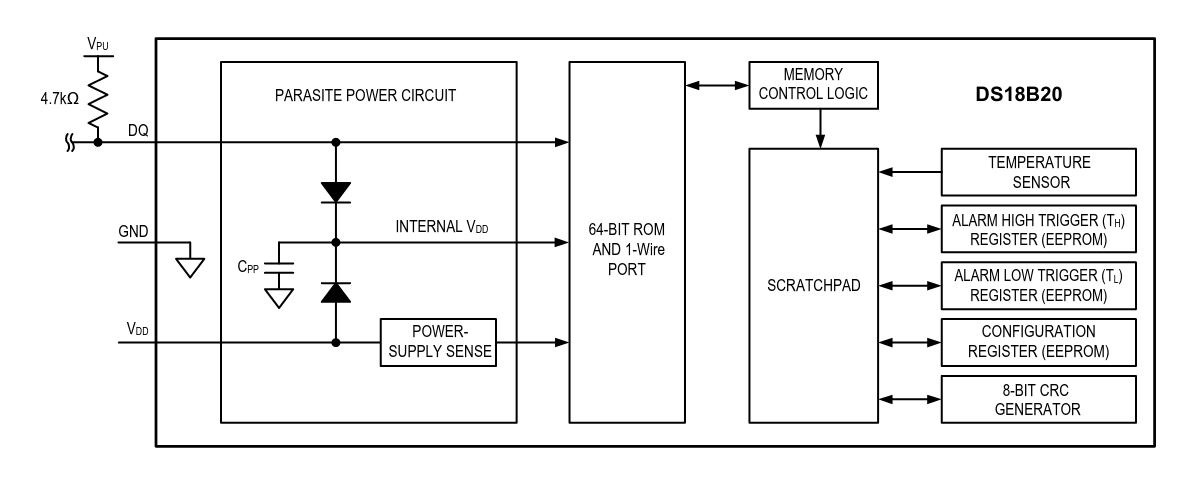
\includegraphics[width=0.8\textwidth]{/home/auan/Project/Report/Images/DS18B20_schem.png}
  \caption{Schematic of the DS18B20 sensor}
  \label{fig:sensorschem}
\end{figure}
\subsubsection{MongoDB}%
\label{ssub:mongodb}
MongoDB is an open source document database suitable for storing time-series data. This acts as the web application back-end and can also store configuration options set by the user. The database can be set up to run a daemonized process, which allows the user to get or set data whenever the server is powered on. Using the Python module PyMongo, it is possible to insert entries using JSON formatting.

\subsubsection{Systemd service}%
\label{ssub:systemd_service}
Many Linux distributions use the Systemd init daemon. While many crucial programs runs in the background by Systemd as default, it is quite straightforward to add a another service that in this case runs the Python temperature reading script. Systemd has several options to restart the service on failure, start without the need to login and redirect \verb|stdout| to the OS log called the \textit{journal}. The latter simplifies tracking how often the service behaves unexpectedly during long timespans.

\begin{lstlisting}[caption={The systemd service managing data collection}, label={systemd}]
[Unit]
# Human readable unit name
Description=Reads serially from '/dev/ttyUSB*' and puts in MongoDB

[Service]
# Command that executes script
ExecStart=/usr/bin/python /home/alarm/Project/serial_temp_to_db.py
# Redirect print() to the Linux journal
Environment=PYTHONUNBUFFERED=1
# Able to notify that the service is ready
Type=notify
Restart=always

[Install]
# Start service at boot
WantedBy=default.target
\end{lstlisting}



\subsubsection{Plotly Dash web application}%
\label{ssub:plotly_dash_web_application}
The web application consists of
\begin{enumerate}
  \item A live graph showing the $n$ most recent data points. It is updated by a timed callback function
  \item A graph showing the historical data of measurements. The user can pick start and stop times from in the span of the registered dates in the database. The data is updated if the page is refreshed.
  \item The user can set alarm levels which sends and alert email if a drastic temperature drop is detected
\end{enumerate}

Dash is an open source data visualization framework that runs in a web application. It is maintained by Plotly and build upon using their graphing software with the same name.

Each website object can be decorated with a callback function that either updates due to a time interval or through user interaction.

In order to utilize the power of Pandas, the data is loaded into a dataframe which allows many types of manipulation in areas such as statistics and signal processing.

Since the data ordered by a timestamp, it is sorted in natural order and the start and stop date can be chosen by the user.
